% Generated by AP Math GOLD PILOT deterministic Python generator.
% input id: 04_circle_tangent_bounds
\documentclass{article}
\usepackage[margin=1cm]{geometry}
\def\pgfsysdriver{pgfsys-dvisvgm.def}
\usepackage{amssymb}
\usepackage{pgfplots}
\pgfplotsset{compat=1.18}
\pagestyle{empty}
\begin{document}
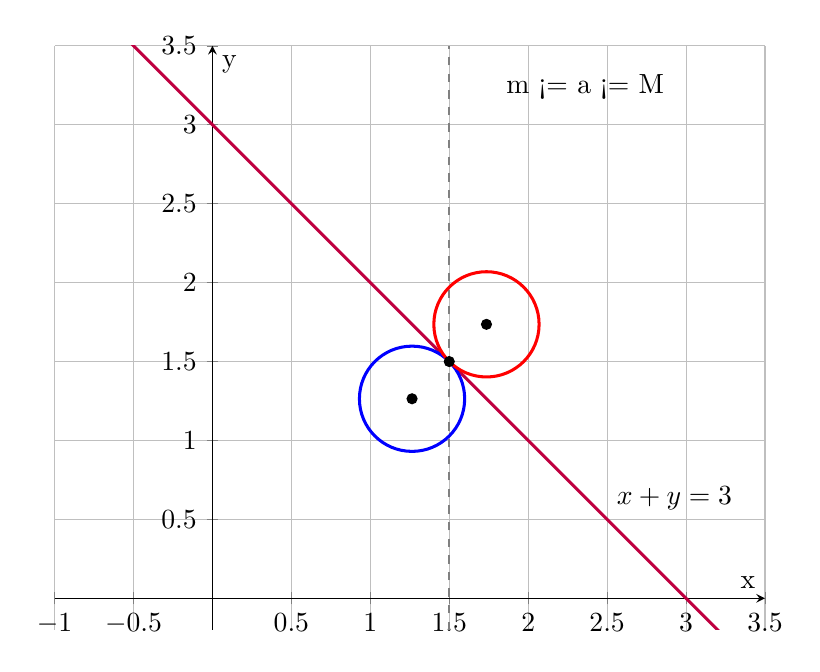
\begin{tikzpicture}
\begin{axis}[width=13cm,height=9cm,axis equal image,axis lines=middle,grid=major,xmin=-1,xmax=3.5,ymin=-0.2,ymax=3.5,xlabel={x},ylabel={y},clip=true]
\addplot[purple, solid, line width=1.1pt] coordinates {(-1,4) (-0.94375,3.94375) (-0.8875,3.8875) (-0.83125,3.83125) (-0.775,3.775) (-0.71875,3.71875) (-0.6625,3.6625) (-0.60625,3.60625) (-0.55,3.55) (-0.49375,3.49375) (-0.4375,3.4375) (-0.38125,3.38125) (-0.325,3.325) (-0.26875,3.26875) (-0.2125,3.2125) (-0.15625,3.15625) (-0.1,3.1) (-0.04375,3.04375) (0.0125,2.9875) (0.06875,2.93125) (0.125,2.875) (0.18125,2.81875) (0.2375,2.7625) (0.29375,2.70625) (0.35,2.65) (0.40625,2.59375) (0.4625,2.5375) (0.51875,2.48125) (0.575,2.425) (0.63125,2.36875) (0.6875,2.3125) (0.74375,2.25625) (0.8,2.2) (0.85625,2.14375) (0.9125,2.0875) (0.96875,2.03125) (1.025,1.975) (1.08125,1.91875) (1.1375,1.8625) (1.19375,1.80625) (1.25,1.75) (1.30625,1.69375) (1.3625,1.6375) (1.41875,1.58125) (1.475,1.525) (1.53125,1.46875) (1.5875,1.4125) (1.64375,1.35625) (1.7,1.3) (1.75625,1.24375) (1.8125,1.1875) (1.86875,1.13125) (1.925,1.075) (1.98125,1.01875) (2.0375,0.9625) (2.09375,0.90625) (2.15,0.85) (2.20625,0.79375) (2.2625,0.7375) (2.31875,0.68125) (2.375,0.625) (2.43125,0.56875) (2.4875,0.5125) (2.54375,0.45625) (2.6,0.4) (2.65625,0.34375) (2.7125,0.2875) (2.76875,0.23125) (2.825,0.175) (2.88125,0.11875) (2.9375,0.0625) (2.99375,0.00625) (3.05,-0.05) (3.10625,-0.10625) (3.1625,-0.1625) (3.21875,-0.21875) (3.275,-0.275) (3.33125,-0.33125) (3.3875,-0.3875) (3.44375,-0.44375) (3.5,-0.5)};
\node[anchor=south west] at (axis cs:-1,4) {$x+y=3$};
\draw[gray, dashed, line width=0.8pt] (axis cs:1.5,-0.2) -- (axis cs:1.5,3.5);
\draw[blue, solid, line width=1.1pt] (axis cs:1.264298,1.264298) circle [radius=0.333333];
\draw[red, solid, line width=1.1pt] (axis cs:1.735702,1.735702) circle [radius=0.333333];
\addplot[only marks,mark=*,mark size=1.8pt,black] coordinates {(1.264298,1.264298)};
\addplot[only marks,mark=*,mark size=1.8pt,black] coordinates {(1.735702,1.735702)};
\addplot[only marks,mark=*,mark size=1.8pt,black] coordinates {(1.5,1.5)};
\node[anchor=south west] at (axis cs:2.5,0.5) {$x+y=3$};
\node[anchor=south west] at (axis cs:1.8,3.1) {m <= a <= M};
\end{axis}
\end{tikzpicture}
\end{document}
